\documentclass[10pt]{article}
\usepackage[a4paper,textwidth=122mm,textheight=193mm,centering]{geometry}
\usepackage[T1]{fontenc}\usepackage{graphicx,booktabs,array,amssymb,amsmath,tabularx,makecell}
\usepackage[font=small,labelfont=bf,labelsep=period]{caption}\renewcommand{\figurename}{Fig.}
\graphicspath{{../figures/}}
\renewenvironment{abstract}{\small\quotation\noindent\textbf{Abstract.} }{\endquotation}
\begin{document}
\begin{center}{\large\bfseries Trust-Weighted Multi-Oracle Validation for Conflicting Land Records: A Simulation Study}\\[2mm] Author name\\ Affiliation\\[6mm]\end{center}
\begin{abstract}
Blockchain land registries make records tamper-evident but cannot check whether the evidence they receive is correct. We study a synthetic pre-commit validation policy that decides whether to record a requested ownership change or escalate it to a person. Each request bundles three simulated checks, record holder, deed registration and pending proceedings, inspired by selected conditions of Gujarat's 2026 mutation fast track. Three offices report on every check. Each report is weighted by the office's assumed authority for that check and by trust learned from verified outcomes; the policy never decides title. In simulation (1,000 requests per run, 100 paired seeds), the hybrid rule cut the false-commit rate from 3.05\% to 1.09\% against majority voting. After the most authoritative office degraded, it beat authority-only weighting (5.52\% vs 6.81\%). Trust-only weighting was safer still but committed fewer valid requests, and a separate veto on reported proceedings never changed a decision. In an exploratory robustness study, 67 of 68 checks of these conclusions held, but errors shared between offices raised every method's false-commit rate sharply.

\par\noindent\textbf{Keywords:}  blockchain oracles $\cdot$ land records $\cdot$ trust and reputation $\cdot$ weighted aggregation $\cdot$ e-governance $\cdot$ simulation\end{abstract}
\section*{1 Introduction}
This paper asks how a ledger should decide, before writing, whether conflicting evidence from several offices is good enough to record a requested ownership change. It does not ask when a land transfer is legally valid: in India, revenue-record entries serve fiscal purposes and do not by themselves confer title [16]. Thakur et al. note that departments hold inconsistent data about the same land, and their blockchain design leaves reconciling those data to pre-deployment work [1].

Gujarat's 2026 ordinance shows how one administration combines such evidence [12]. A mutation from a registered sale deed is certified the same day only if the record of rights has not changed for a year, everyone named in it executed the deed, and no dispute or proceeding about the land is pending; otherwise the normal notice route applies. Our model borrows the shape of this rule, not its content: it simulates checks loosely inspired by the last two conditions, plus deed registration.

Blockchains, including permissioned platforms such as Hyperledger Fabric [2], have been proposed as tamper-evident land registries [1], [5]--[7], [15]. Data enter a chain through oracles, which bring back trust in third parties [3], [8]. Oracle networks combine reporters by voting or reputation [4], [10], and truth-discovery methods estimate source reliability from conflicting reports [13], [14]. Land evidence adds two complications: each office is the natural source for a different fact, and a pending proceeding plausibly calls for review rather than a vote.

We ask: does combining claim-specific authority with learned reliability reduce false commits compared with majority, authority-only and trust-only weighting (RQ1)? What happens when the authoritative office degrades or authority is misassigned (RQ2)? How do outages and a coverage requirement trade false commits for escalations (RQ3)? Does a separate veto on reported proceedings change decisions (RQ4)? How do delayed, incomplete labels affect learned trust (RQ5)? Our contributions are a pre-commit policy for a three-check request bundle; a component-level comparison of five mechanisms on identical simulated worlds under a protocol frozen before the final runs, with two pre-registered exploratory addenda; and evidence on when each component helps and where the approach is fragile.

\section*{2 Related Work}
Thakur et al. [1] sketch a design whose nodes include revenue, registration, survey and court participants. Consensus validates transactions, not the accuracy of the underlying records, and consolidating inconsistent departmental data is deferred [1, Secs. 3.4, 6, 7.1]. Soner et al. [5], Shuaib et al. [6] and Sahai and Pandey [7] use smart contracts at registry stages. Khanna et al. [15] model six administrative roles with role-aware endorsement in Hyperledger Fabric. Caldarelli notes that contracting and law may need a hierarchy of oracles so that illegal agreements can be reverted, without defining one [3, Sec. 5]. Oracle surveys compare trust mechanisms based on voting and reputation [4], [8]. Truth discovery jointly estimates truth and source reliability without labels [13], and DecenTruth applies it inside an oracle network [14]. Our trust score is a simple reputation score [11], updated only from verified outcomes and combined with a fixed, claim-specific authority prior. Table 1 compares the approaches. Among these sources we found no pre-commit rule that combines claim-specific authority with learned per-check reliability, escalates rather than rejects, and is evaluated against hidden ground truth; this claim is bounded to the sources listed.

% Auto-generated by paper_assets/build_assets.py from saved results -- do not edit numbers by hand.
% Preamble needs: \usepackage{booktabs,array,tabularx,makecell}
\begin{table}[tb]
\centering
\caption{Comparison with related work}\label{tab:related}
\footnotesize
\setlength{\tabcolsep}{2pt}
\renewcommand{\arraystretch}{1.1}
\begin{tabularx}{\textwidth}{@{}>{\raggedright\arraybackslash}p{2.0cm}*{7}{>{\raggedright\arraybackslash}X}@{}}
\toprule
Work & Land records & Multi-source & Per-claim authority & Learned trust & Pre-commit conflict check & Escalates & Ground truth \\
\midrule
Thakur et al. [1] & yes & yes (nodes) & no & no & no (deferred) & manual & no \\
Soner et al. [5]$^\dagger$ & yes & yes & ? & ? & ? & ? & ? \\
Shuaib et al. [6]$^\dagger$ & yes & ? & ? & ? & ? & ? & ? \\
Sahai, Pandey [7]$^\dagger$ & yes & ? & ? & ? & ? & ? & ? \\
Khanna et al. [15]$^\ddagger$ & yes & yes (6 roles) & role-based & n.s. & n.s. & n.s. & n.s. \\
Chainlink [10] & no & yes (nodes) & no & reput. & aggreg. & no & no \\
Truth discovery [13] & no & yes & no & yes (unsup.) & yes & no & --- \\
DecenTruth [14]$^\ddagger$ & no & yes & no & yes (unsup.) & yes & n.s. & sim. \\
This work & synthetic & yes (3) & yes & yes (labels) & yes & yes & yes \\
\bottomrule
\end{tabularx}
\par\smallskip
\parbox{\textwidth}{\scriptsize $^\dagger$ Full text not yet read; ? = not determined. $^\ddagger$ Compared at abstract level only. n.s. = not stated in the abstract; unsup. = estimated without labels; reput. = reputation; aggreg. = aggregation of node reports; sim. = simulation; --- = not applicable to a survey.}
\end{table}

\section*{3 Model}
The validator records a request only when all three checks pass on their own evidence; otherwise it escalates (Fig. 1).

\begin{figure}[tb]\centering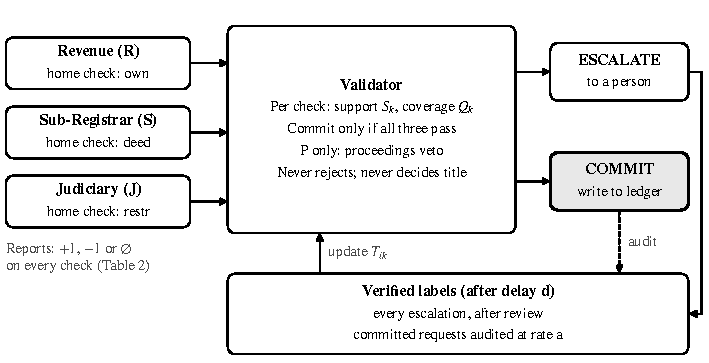
\includegraphics[width=\textwidth]{fig1_system.pdf}\caption{Validation loop. Three offices report on three checks, the validator commits a request only when all three checks pass and otherwise escalates it, and verified labels update trust.}\end{figure}
A request x carries checks k $\in$ {own, deed, restr}, each with hidden truth $g\_k(x)$ $\in$ {+1, --1}; it is valid only when all three are +1. Revenue (R), Sub-Registrar (S) and Judiciary (J) each report +1, --1 or $\varnothing$ (no response) on every check. Off-home reports are less accurate. The reports are simulated signals with illustrative meanings (Table S1), not claims about what real offices hold. Authority $A(i,k)$ is an assumption reflecting which office is the natural source for each check (Table 2). Each office holds one trust score per check, $T\_{ik}$, starting at 0.5 and updated only from verified labels:

\[T_{ik} \leftarrow (1-\alpha)\,T_{ik} + \alpha\,\mathbf{1}[\,r_{ik}(x) = g_k(x)\,], \qquad \alpha = 0.1\]
% Auto-generated by paper_assets/build_assets.py from saved results -- do not edit numbers by hand.
% Preamble needs: \usepackage{booktabs,array,tabularx,makecell}
\begin{table}[tb]
\centering
\caption{Claim-specific authority $A(i,k)$ (modelling assumption)}\label{tab:authority}
\small
\setlength{\tabcolsep}{3pt}
\renewcommand{\arraystretch}{1.1}
\begin{tabular}{@{}lccc@{}}
\toprule
Check & Revenue & Sub-Registrar & Judiciary \\
\midrule
own & 1.0 & 0.6 & 0.4 \\
deed & 0.6 & 1.0 & 0.4 \\
restr & 0.2 & 0.2 & 1.0 \\
\bottomrule
\end{tabular}
\end{table}

With weights $w\_{ik}$ = $A(i,k)$$\cdot$$T\_{ik}$ and $R\_k(x)$ the offices that reported on check k, support and coverage are

\[S_k(x) = \frac{\sum_{i \in R_k(x)} w_{ik}\,\mathbf{1}[r_{ik}(x) = +1]}{\sum_{i \in R_k(x)} w_{ik}}, \qquad Q_k(x) = \frac{\sum_{i \in R_k(x)} w_{ik}}{\sum_{i} w_{ik}}.\]
A request escalates if no office responds, if (with the veto) the Judiciary reports a proceeding and $T\_{J,\mathrm{restr}}$ $\geq$ 0.6, or if any check fails its coverage gate or has $S\_k$ < $\theta$ = 0.65; otherwise it commits. When the Judiciary reports a proceeding, $S\_\mathrm{restr}$ $\leq$ (0.2 + 0.2)/(0.2 + 0.2 + 1.0 $\times$ 0.6) = 0.4 < $\theta$, so the weighted rule already escalates every case the veto would catch.

Table 3 follows one invalid request in which a pending proceeding is visible only to the Judiciary. Majority voting and trust-only weighting commit it; authority-aware weighting gives the Judiciary most of the weight on restr and escalates.

% Auto-generated by paper_assets/build_assets.py from saved results -- do not edit numbers by hand.
% Preamble needs: \usepackage{booktabs,array,tabularx,makecell}
\begin{table}[tb]
\centering
\caption{Worked example: request 123 in S5a, seed 1, with a pending proceeding visible only to the Judiciary}\label{tab:example}
\footnotesize
\setlength{\tabcolsep}{3pt}
\renewcommand{\arraystretch}{1.1}
\begin{tabularx}{\textwidth}{@{}lcl>{\raggedright\arraybackslash}Xl@{}}
\toprule
Mechanism & \makecell{Support for \\ `clear' on restr} & Decision & Reason code & Outcome \\
\midrule
B1 Majority & 2 of 3 clear & COMMIT & --- & false commit \\
B2 Authority-only & 0.286 & ESCALATE & restr: low support & escalated \\
B3 Trust-only & 0.666 & COMMIT & --- & false commit \\
P$-$V Hybrid & 0.285 & ESCALATE & restr: low support & escalated \\
P Hybrid + veto & veto first & ESCALATE & veto: proceeding reported & escalated \\
\bottomrule
\end{tabularx}
\par\smallskip
\parbox{\textwidth}{\scriptsize Truth: own pass, deed pass, restr pending (request invalid). Reports (own, deed, restr): R: +1 +1 +1; S: $-$1 +1 +1; J: +1 +1 $-$1. Trust under ideal feedback at that point: R, S and J on restr $\approx$ 1.00; $\theta$ = 0.65.}
\end{table}

\section*{4 Experimental Setup}
Each run has 1,000 requests. Checks fail independently with probability 0.12, 0.12 and 0.08 (28.8\% of requests invalid). An office reports correctly with probability 0.95 on its home check and 0.75 otherwise, and is down with probability 0.03. All values are assumptions. Tables 4 and 5 list the scenarios and mechanisms; every mechanism requires all three checks to pass. B1 uses a count gate, the weighted mechanisms a weighted gate; these are not the same rule, and an exploratory ablation separates them (Sect. 5.4). Main results use ideal feedback (every label revealed at once), an upper bound for the trust-based mechanisms. The realistic regime labels escalated requests plus an audit of commits at rate a $\in$ {0, 0.05, 0.2}, with delay d $\in$ {0, 50, 200}.

% Auto-generated by paper_assets/build_assets.py from saved results -- do not edit numbers by hand.
% Preamble needs: \usepackage{booktabs,array,tabularx,makecell}
\begin{table}[tb]
\centering
\caption{Scenarios; each changes one setting from S1}\label{tab:scenarios}
\footnotesize
\setlength{\tabcolsep}{3pt}
\renewcommand{\arraystretch}{1.1}
\begin{tabularx}{\textwidth}{@{}l>{\raggedright\arraybackslash}Xc@{}}
\toprule
Scenario & Change from S1 & RQ \\
\midrule
S1 Aligned & None: authority matches each office's most accurate check & 1 \\
S2 Degraded & From request 251, Revenue accuracy 0.50 on all checks & 2 \\
S3 Misaligned & On own, Revenue 0.75 and Sub-Registrar 0.95; authority unchanged & 2 \\
S4 Low availability & Outage probability 0.25 per office per request & 3 \\
S5a Proceedings stress & Revenue and Sub-Registrar always report `clear' on restr & 4 \\
S5b Alt. authority & As S5a, with A(R, restr) = A(S, restr) = 0.6 & 4 \\
\bottomrule
\end{tabularx}
\end{table}

% Auto-generated by paper_assets/build_assets.py from saved results -- do not edit numbers by hand.
% Preamble needs: \usepackage{booktabs,array,tabularx,makecell}
\begin{table}[tb]
\centering
\caption{Mechanisms compared}\label{tab:mechanisms}
\footnotesize
\setlength{\tabcolsep}{3pt}
\renewcommand{\arraystretch}{1.1}
\begin{tabularx}{\textwidth}{@{}ll>{\raggedright\arraybackslash}X>{\raggedright\arraybackslash}Xcc@{}}
\toprule
Mechanism & Weight & Pass rule per check & Coverage gate & Veto & Learns \\
\midrule
B1 Majority & 1 & $>$ half of responders & $\geq$ 2 of 3 responded & no & no \\
B2 Authority-only & $A(i,k)$ & $S_k$ $\geq$ $\theta$ & $Q_k$ $\geq$ 0.5 & no & no \\
B3 Trust-only & $T_{ik}$ & $S_k$ $\geq$ $\theta$ & $Q_k$ $\geq$ 0.5 & no & yes \\
P$-$V Hybrid & $A(i,k)$$\cdot$$T_{ik}$ & $S_k$ $\geq$ $\theta$ & $Q_k$ $\geq$ 0.5 & no & yes \\
P Hybrid + veto & $A(i,k)$$\cdot$$T_{ik}$ & $S_k$ $\geq$ $\theta$ & $Q_k$ $\geq$ 0.5 & yes & yes \\
\bottomrule
\end{tabularx}
\end{table}

We report the false-commit rate (FCR, false commits $\div$ commits) and valid-commit coverage (VCC, valid commits $\div$ valid requests). Eight hypotheses were pre-specified and tested as paired differences across seeds with 95\% t-intervals. Seven were Holm-adjusted together, with $\Delta$ = 0.5 percentage points as the minimum difference of interest. A stopping rule raised the seed count to its cap of 100. Table S3 records which results are pre-specified and which exploratory; Table S4 lists five analysis choices outside the protocol.

\section*{5 Results}
Tables 6 and 7 give the pre-specified results under ideal feedback.

% Auto-generated by paper_assets/build_assets.py from saved results -- do not edit numbers by hand.
% Preamble needs: \usepackage{booktabs,array,tabularx,makecell}
\begin{table}[tb]
\centering
\caption{False-commit rate (FCR) and valid-commit coverage (VCC), \%, mean over 100 seeds, ideal feedback}\label{tab:main}
\footnotesize
\setlength{\tabcolsep}{3pt}
\renewcommand{\arraystretch}{1.1}
\begin{tabular}{@{}l*{8}{c}@{}}
\toprule
 & \multicolumn{2}{c}{S1 Aligned} & \multicolumn{2}{c}{S2 Degraded} & \multicolumn{2}{c}{S3 Misaligned} & \multicolumn{2}{c}{S4 Low avail.} \\
\cmidrule(lr){2-3}\cmidrule(lr){4-5}\cmidrule(lr){6-7}\cmidrule(l){8-9}
Mechanism & FCR & VCC & FCR & VCC & FCR & VCC & FCR & VCC \\
\midrule
B1 Majority & 3.05 & 73.2 & 6.34 & 56.3 & 3.03 & 73.2 & 2.87 & 44.6 \\
B2 Authority-only & 1.15 & 71.5 & 4.63 & 44.8 & 2.09 & 60.0 & 1.64 & 45.9 \\
B3 Trust-only & 1.06 & 61.7 & 2.54 & 42.2 & 1.03 & 61.7 & 1.35 & 39.5 \\
Hybrid (P$-$V = P) & 1.09 & 68.7 & 3.86 & 44.2 & 1.50 & 57.9 & 1.13 & 31.8 \\
\bottomrule
\end{tabular}
\par\smallskip
\parbox{\textwidth}{\scriptsize Between-seed SD: FCR 0.45--1.23, VCC 1.7--2.0. P and P$-$V made identical decisions in every run of S1--S4.}
\end{table}

% Auto-generated by paper_assets/build_assets.py from saved results -- do not edit numbers by hand.
% Preamble needs: \usepackage{booktabs,array,tabularx,makecell}
\begin{table}[tb]
\centering
\caption{Pre-specified paired comparisons (100 seeds; percentage points; breaches per 1,000 requests)}\label{tab:primary}
\footnotesize
\setlength{\tabcolsep}{3pt}
\renewcommand{\arraystretch}{1.1}
\begin{tabularx}{\textwidth}{@{}l>{\raggedright\arraybackslash}Xccc>{\raggedright\arraybackslash}p{1.55cm}@{}}
\toprule
ID & Metric: comparison (scenario) & Difference [95\% CI] & Half-width & Holm p & Reading \\
\midrule
H1a & FCR: P$-$V $-$ B1 (S1) & $-$1.96 [$-$2.12, $-$1.81] & 0.16 & <0.001 & lower \\
H1b & FCR: P$-$V $-$ B2 (S1) & $-$0.06 [$-$0.09, $-$0.03] & 0.03 & <0.001 & lower, < $\Delta$ \\
H2a & FCR: P$-$V $-$ B2 (S2, 251--1000) & $-$1.28 [$-$1.49, $-$1.08] & 0.20 & <0.001 & lower \\
H2b & VCC: P$-$V $-$ B3 (S2, 251--1000) & +0.30 [$-$0.13, +0.72] & 0.42$^\dagger$ & 0.25 & no clear diff. \\
H2c & FCR: P$-$V $-$ B2 (S3) & $-$0.60 [$-$0.67, $-$0.52] & 0.08 & <0.001 & lower \\
H3 & VCC: P$-$V $-$ B1 (S4) & $-$12.82 [$-$13.10, $-$12.54] & 0.28$^\dagger$ & --- & lower (descr.) \\
H4 & Breaches: P $-$ P$-$V (S5b) & 0 & 0.00 & 1.00 & identical \\
H5 & FCR: P under F1 $-$ F0 (S2) & $-$0.13 [$-$0.25, $-$0.005] & 0.12 & 1.00 & not supported \\
\bottomrule
\end{tabularx}
\par\smallskip
\parbox{\textwidth}{\scriptsize $^\dagger$ Above the precision target $\Delta$/2 at the 100-seed cap. H3 is descriptive. H5 was one-sided (F1 higher).}
\end{table}

\textbf{RQ1.} The hybrid's FCR was 1.96 points below majority's, about 5 false commits per 1,000 requests instead of 16, at the cost of 489 valid commits instead of 521. Against authority-only, the 0.06-point difference was below $\Delta$: when authority matches accuracy, as designed in S1, learned trust adds little.

\textbf{RQ2.} After Revenue degraded (requests 251--1000), the hybrid's FCR was 5.52\% against 6.81\% for authority-only. With authority misassigned (S3), it was 0.60 points lower. Trust-only, however, had the lowest FCR in S2: Revenue's authority of 1.0 keeps its weight high even when its trust falls to about 0.46. Fig. 2 shows the threshold trade-off: the hybrid is best at low thresholds, trust-only between $\theta$ $\approx$ 0.6 and 0.85.

\begin{figure}[tb]\centering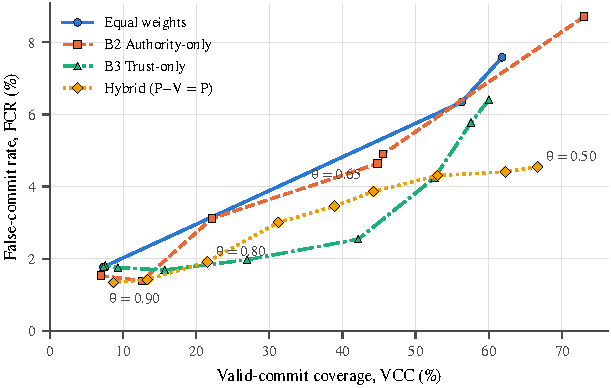
\includegraphics[]{fig2_threshold_tradeoff.pdf}\caption{Commit-threshold trade-off after Revenue degrades (S2): false-commit rate against valid-commit coverage as $\theta$ varies from 0.50 to 0.90 in steps of 0.05 (means over 100 seeds, ideal feedback)}\end{figure}
\textbf{RQ3--RQ5.} With 25\% outages the hybrid kept FCR at 1.13\% but committed only 31.8\% of valid requests, against 44.6\% for majority. The veto never changed a decision (H4), because the Judiciary's learned trust stayed outside the narrow window in which it could act. In the proceedings stress test, breaches per 1,000 requests were 50.6 for majority, 32.8 for trust-only and 2.2 for the hybrid. Realistic feedback did not raise FCR (H5 not supported; Fig. S1). Trust learned mostly from contested requests, and this selection bias happened to help.

\subsection*{5.4 Exploratory analyses}
A coverage-gate ablation (addendum A1, Table S2) re-ran every mechanism under one common two-of-three gate. The hybrid's FCR stayed 1.85 points below majority's, so the gain comes from weighting. Its coverage matched majority's in S1 and exceeded it by 8.4 points under outages, so the main-study coverage gap came from the stricter weighted gate.

A robustness study (addendum A2, committed before running with a commitment to report every result) varied one assumption at a time. Of 68 checks of the main conclusions, 67 held and none reversed (Table 8, Fig. 3). The exception was the hybrid against authority-only after degradation at off-home accuracy 0.60 (--0.15 points, CI [--0.39, +0.09]). Shared errors kept the ranking but raised every rate: at a shared error rate of 0.20, the hybrid's FCR in S1 rose from 1.09\% to 8.33\%, against 11.93\% for majority.

% Auto-generated by paper_assets/build_assets.py from saved results -- do not edit numbers by hand.
% Preamble needs: \usepackage{booktabs,array,tabularx,makecell}
\begin{table}[tb]
\centering
\caption{Exploratory robustness study A2: levels at which each main conclusion holds, with the range of FCR differences in points}\label{tab:robustness}
\footnotesize
\setlength{\tabcolsep}{3pt}
\renewcommand{\arraystretch}{1.1}
\begin{tabularx}{\textwidth}{@{}>{\raggedright\arraybackslash}Xcccc@{}}
\toprule
Factor varied & C1 (S1) & C1 (S2) & C2 & C3 \\
\midrule
Off-home accuracy 0.60--0.85 & \makecell{4/4 \\ ($-$6.2 to $-$0.4)} & \makecell{4/4 \\ ($-$4.9 to $-$1.4)} & \makecell{3/4 \\ ($-$1.6 to $-$0.2)} & \makecell{4/4 \\ ($-$1.3 to $-$0.8)} \\
Home accuracy 0.85--0.95 & \makecell{3/3 \\ ($-$2.0 to $-$0.9)} & \makecell{3/3 \\ ($-$2.5 to $-$1.6)} & \makecell{3/3 \\ ($-$1.3 to $-$1.1)} & \makecell{3/3 \\ ($-$1.9 to $-$1.3)} \\
Shared R+S errors $\rho$ = 0--0.20 & \makecell{4/4 \\ ($-$3.6 to $-$2.0)} & \makecell{4/4 \\ ($-$3.6 to $-$2.5)} & \makecell{4/4 \\ ($-$2.0 to $-$1.3)} & \makecell{4/4 \\ ($-$5.0 to $-$1.3)} \\
Label noise e = 0--0.10, F0 & --- & \makecell{4/4 \\ ($-$2.5 to $-$2.4)} & \makecell{4/4 \\ ($-$1.3 to $-$1.1)} & \makecell{4/4 \\ ($-$1.3 to $-$1.2)} \\
Label noise e = 0--0.10, F1 & --- & \makecell{4/4 \\ ($-$2.6 to $-$2.5)} & \makecell{4/4 \\ ($-$1.6 to $-$1.4)} & \makecell{4/4 \\ ($-$0.9 to $-$0.8)} \\
\bottomrule
\end{tabularx}
\par\smallskip
\parbox{\textwidth}{\scriptsize C1: hybrid below majority. C2: hybrid below authority-only after degradation (requests 251--1000). C3: trust-only below hybrid (S2). Holds: the 95\% CI excludes 0 with the main-study sign. No conclusion reversed.}
\end{table}

\begin{figure}[tb]\centering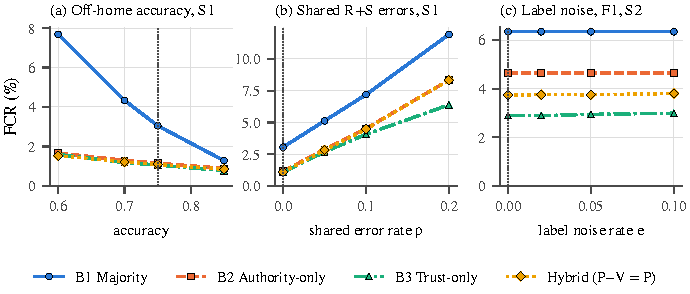
\includegraphics[]{fig3_robustness.pdf}\caption{Exploratory robustness study A2 (100 seeds): false-commit rate by mechanism as (a) off-home accuracy, (b) the shared error rate of Revenue and Sub-Registrar and (c) label noise vary; dotted lines mark the main-study settings}\end{figure}
\section*{6 Discussion}
Under the stated assumptions, the results support weighting conflicting evidence rather than counting votes, but not calling the hybrid the best rule. Authority-aware weighting gives most of the gain over majority voting, independent of the coverage gate and across every robustness level tested. Learned trust adds protection when authority is wrong or degrades, under ideal feedback. Multiplying authority by trust leaves a degraded high-authority office with substantial weight, which is why trust-only was safer after degradation; an above-chance trust transform is left to future work. The veto's null result is limited to the tested configurations: the model abstracts what a reported proceeding means and whether it binds the change. The coverage gate is a policy lever that trades a little safety for a lot of coverage.

The main weakness is shared errors. Weighting cannot detect two offices that are confidently wrong together, so a real deployment would need independent evidence for at least one check. Every weighted mechanism also escalated about half of all requests in S1, a heavy review load. Threats to validity: the data are synthetic and all rates are assumed; the model omits record stability and does not decide title; outages and most errors are independent; main results assume immediate, error-free labels; S1 aligns authority with accuracy by design. Two intervals missed their precision target, and A1, A2 and five analysis choices are exploratory or outside the protocol.

\section*{7 Conclusion}
A pre-commit policy that weights each office's report by claim-specific authority and learned trust cut false commits about threefold against majority voting in simulation. The gain held under a common coverage gate and across all robustness levels tested. Learned trust helped when authority degraded or was misassigned, although trust-only weighting was safer still at a cost in coverage, and a separate proceedings veto added nothing in the configurations tested. Future work: detecting copied records, an above-chance trust transform, parameters grounded in verified Gujarat sources, adversarial sources and chaincode integration. Code, data and supplementary material are available at https://github.com/HetSagar/trust\_aware\_oracle\_consensus\_for\_blockchain.

\section*{References}\footnotesize
\begin{enumerate}
\item V. Thakur, M. N. Doja, Y. K. Dwivedi, T. Ahmad, and G. Khadanga, "Land records on Blockchain for implementation of Land Titling in India," Int. J. Inf. Manage., vol. 52, Art. no. 101940, Jun. 2020, doi: 10.1016/j.ijinfomgt.2019.04.013.
\item E. Androulaki et al., "Hyperledger Fabric: A distributed operating system for permissioned blockchains," in Proc. 13th EuroSys Conf., Porto, Portugal, Apr. 2018, doi: 10.1145/3190508.3190538.
\item G. Caldarelli, "Understanding the blockchain oracle problem: A call for action," Information, vol. 11, no. 11, Art. no. 509, Oct. 2020, doi: 10.3390/info11110509.
\item H. Al-Breiki, M. H. U. Rehman, K. Salah, and D. Svetinovic, "Trustworthy blockchain oracles: Review, comparison, and open research challenges," IEEE Access, vol. 8, pp. 85675–85685, 2020, doi: 10.1109/ACCESS.2020.2992698.
\item S. Soner, R. Litoriya, and P. Pandey, "Exploring blockchain and smart contract technology for reliable and secure land registration and record management," Wireless Pers. Commun., vol. 121, no. 4, pp. 2495–2509, Dec. 2021, doi: 10.1007/s11277-021-08833-1.
\item M. Shuaib, S. M. Daud, S. Alam, and W. Z. Khan, "Blockchain-based framework for secure and reliable land registry system," TELKOMNIKA, vol. 18, no. 5, pp. 2560–2571, Oct. 2020, doi: 10.12928/TELKOMNIKA.v18i5.15787.
\item A. Sahai and R. Pandey, "Smart contract definition for land registry in blockchain," in Proc. IEEE 9th Int. Conf. Commun. Syst. Netw. Technol. (CSNT), Gwalior, India, 2020, pp. 230–235, doi: 10.1109/CSNT48778.2020.9115752.
\item A. Hassan, I. Makhdoom, W. Iqbal, A. Ahmad, and A. Raza, "From trust to truth: Advancements in mitigating the blockchain oracle problem," J. Netw. Comput. Appl., vol. 217, Art. no. 103672, Aug. 2023, doi: 10.1016/j.jnca.2023.103672.
\item S. K. Lo, X. Xu, M. Staples, and L. Yao, "Reliability analysis for blockchain oracles," Comput. Electr. Eng., vol. 83, Art. no. 106582, 2020. [VERIFY DOI]
\item L. Breidenbach et al., "Chainlink 2.0: Next steps in the evolution of decentralized oracle networks," Chainlink Labs, white paper v1.0, Apr. 15, 2021. [Online]. Available: https://research.chain.link/whitepaper-v2.pdf
\item A. Josang, R. Ismail, and C. Boyd, "A survey of trust and reputation systems for online service provision," Decis. Support Syst., vol. 43, no. 2, pp. 618–644, Mar. 2007, doi: 10.1016/j.dss.2005.05.019.
\item Government of Gujarat, Revenue Dept., "The Gujarat Land Revenue (Amendment) Ordinance, 2026," Gujarat Ordinance No. 1 of 2026, Gujarat Government Gazette, Extraordinary, Part IV, Extra No. 6, Mar. 31, 2026. [VERIFY: whether replaced by an Act]
\item Y. Li et al., "A survey on truth discovery," arXiv:1505.02463, 2015. [VERIFY: journal version]
\item Y. Xiao, N. Zhang, W. Lou, and Y. T. Hou, "A decentralized truth discovery approach to the blockchain oracle problem," in Proc. IEEE INFOCOM, 2023, pp. 1–10. [VERIFY DOI]
\item A. Khanna, P. Singh, and P. K. Angra, "Blockchain-enabled e-governance framework for secure and transparent land record management," Int. Res. J. Multidiscip. Technovation, vol. 8, no. 4, pp. 73–90, 2026, doi: 10.54392/irjmt2645.
\item Jitendra Singh v. State of M.P., 2021 SCC OnLine SC 802 (Sept. 6, 2021); see also Tarachandra v. Bhawarlal, 2025 INSC 1485. [VERIFY: judgment texts]
\end{enumerate}
LNCS uses its own reference style (numbered, Springer format). Convert these IEEE-style entries with the template's bibliography style; keep the DOIs.


\end{document}
